\documentclass[border=4pt]{standalone}
\usepackage{amsmath,amssymb}
\usepackage{tikz}
\usetikzlibrary{arrows.meta}
\begin{document}
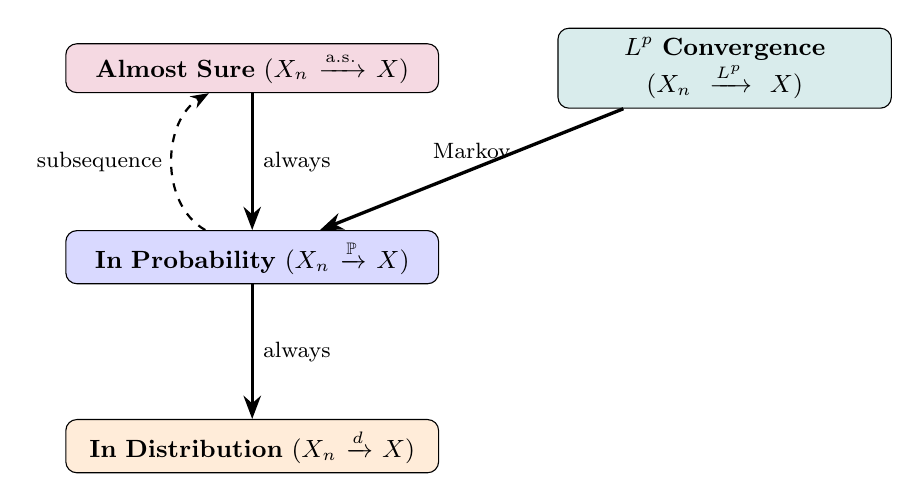
\begin{tikzpicture}[font=\small, >=Stealth]
  \node[draw, rounded corners, fill=purple!15, text width=4.5cm, align=center] (AS) at (0, 2.4)
    {\textbf{Almost Sure} ($X_n \xrightarrow{\mathrm{a.s.}} X$)};
  \node[draw, rounded corners, fill=teal!15, text width=4.0cm, align=center] (LP) at (6.0, 2.4)
    {\textbf{$L^p$ Convergence} ($X_n \xrightarrow{L^p} X$)};
  \node[draw, rounded corners, fill=blue!15, text width=4.5cm, align=center] (PR) at (0, 0.0)
    {\textbf{In Probability} ($X_n \xrightarrow{\mathbb{P}} X$)};
  \node[draw, rounded corners, fill=orange!15, text width=4.5cm, align=center] (DI) at (0, -2.4)
    {\textbf{In Distribution} ($X_n \xrightarrow{d} X$)};

  \draw[->, very thick] (AS) -- node[right, font=\footnotesize] {always} (PR);
  \draw[->, very thick] (LP) -- node[above, font=\footnotesize] {Markov} (PR);
  \draw[->, very thick] (PR) -- node[right, font=\footnotesize] {always} (DI);
  \draw[->, thick, dashed] (PR) to[out=150, in=210] node[left, font=\footnotesize] {subsequence} (AS);
\end{tikzpicture}
\end{document}